\documentclass{article}
\usepackage{tikz}
\usetikzlibrary{arrows.meta}

\begin{document}

\begin{figure}[h]
    \centering
    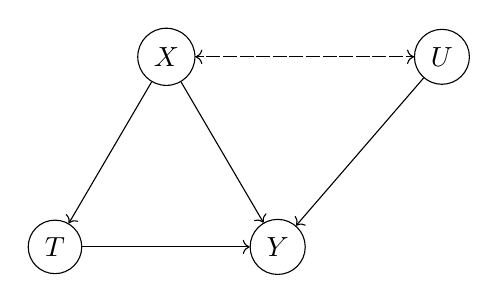
\begin{tikzpicture}[node distance=2cm, auto]
        \node [circle, draw] (X) {$X$};
        \node [circle, draw, right of=X, xshift=1.5cm] (U) {$U$};
        \node [circle, draw, below left of=X, yshift=-1cm] (T) {$T$};
        \node [circle, draw, below right of=X, yshift=-1cm] (Y) {$Y$};

        \draw[->] (X) -- (T);
        \draw[->] (X) -- (Y);
        \draw[->] (U) -- (Y);
        \draw[->] (T) -- (Y);

        \draw[dashed, ->] (X) -- (U);
        \draw[dashed, ->] (U) -- (X);

        \node at (U) [right] {};
    \end{tikzpicture}
    \caption{Example causal graph with hidden confounding. $X$: Observed covariates, $U$: Hidden confounders, $T$: Treatment, $Y$: Outcome. Direct edges denote causal relations and the bidirectional edge signifies possible correlation.}
    \label{fig:causal_graph_hidden_confounding}
\end{figure}

\end{document}